\documentclass{article}
\usepackage[utf8]{inputenc}
\usepackage{geometry}
 \geometry{
 a4paper,
 total={170mm,257mm},
 left=20mm,
 top=20mm,
 }
 \usepackage{graphicx}
 \graphicspath{{Pics/}}
 \usepackage{titling}
 \title{Simulating capital return and income growth to explore their impact on wealth inequality
}
\author{Haoran Jie hj376}
\date{January 2023}
 
 \usepackage{fancyhdr}
\fancypagestyle{plain}{%  the preset of fancyhdr 
    \fancyhead[L]{Tick4}
    \fancyhead[R]{\theauthor}
}
\makeatletter
\def\@maketitle{%
  \newpage
  \null
  \vskip 1em%
  \begin{center}%
  \let \footnote \thanks
    {\LARGE \@title \par}%
    \vskip 1em%
    %{\large \@date}%
  \end{center}%
  \par
  \vskip 1em}
\makeatother

\usepackage{lipsum}  
\usepackage{cmbright}

\begin{document}

\maketitle


\section*{Goals}
Argued by the economist Thomas Piketty in his book \textit{Capital in the Twenty-first Century}, the growth of income from capital (i.e. investments, property, etc.)\footnote{In this study we simplify the situation by assuming capital to be the current wealth} has been outpacing economic growth, leading to increased inequality. This report gather, simulate, and analyse data to test the validity of Piketty's theory and to understand the causes and implications of increasing inequality.

\section*{Methodology}
To investigate this idea, we will create a simple model of the economy by assigning each individual(1000 in total) a per-timestep income, 
which will be randomly chosen a priori. We will then incorporate return on capital into the model by multiplying wealth by a growth factor every timestep.
Additionally, we will normalize wealth every timestep to prevent unbounded growth.\\
To measure the results of our simulation, we will use the \textbf{Gini coefficient}, which measures the level of inequality in a society, 
and a \textbf{mobility measure}, which calculates the proportion of people who moved by more than one quintile.\\
We will run simulations with different ratios of return on capital to growth due to income (0.7 and 2) and compare the results to see if increasing the return on capital leads to higher inequality.





% 1000 individuals randomly assigned per-timestep income
% Return on capital growth factor
% Gini coeficient to measure inequality
% Also measure economic mobility because "some degree of inequality might be acceptible if economic mobility were high"
% Incorporate exchange model to allow for certain level of uncertainty (The extension for tick 1)\\

\section*{Result}
Our simulation results show that as the ratio of return on capital to growth due to income increases, 
the Gini coefficient also increases as iteration goes through, indicating higher levels of inequality. 

\vspace{0.3cm}
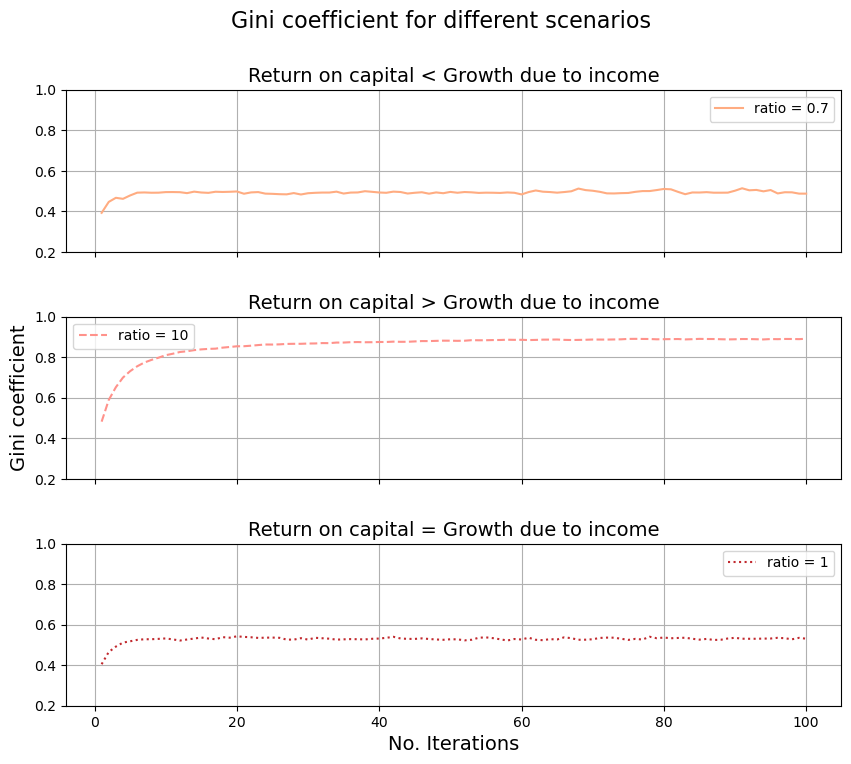
\includegraphics[width=7cm,height=6cm]{ratio_comparison.png}


\section*{Conclusion}


\end{document}
